\newpage
\subsection{Introduction}
Nowadays, web applications are dominating online systems.
From Google, to Facebook and others, web applications are widely deployed across organizations and continuously accessed by end-users, both for their personal and professional daily tasks.
In practice, the development of these web applications heavily rely on a wide ecosystem of \emph{web frameworks}, which are intended to ease and foster the development process.
However, once deployed, the applications developed with such web frameworks do not exhibit the same performances, as reported by the \emph{Web Framework Benchmarks} periodically published by the \textsc{TechEmpower} company.\footnote{\url{https://www.techempower.com/benchmarks}}
Thanks to such benchmarks, developers can take informed decisions on the most performing technology to adopt to implement their web applications.
Unfortunately, one can regret that developers and benchmark providers focus mostly on popularity and performance criteria when picking a web framework, with less considerations for the resource consumption implications of their choice.
This is all the more regrettable that cloud providers are more and more adopted by developers to host these web applications.
While cloud providers offer a convenient elastic provision of resources to scale according to application requirements, this convenience may induce critical cost for their business.
% , their pricing model focuses on this resource consumption by charging the application owner.

Beyond the economical cost of web applications, one can also question the more global impact of web applications on worldwide carbon emissions.
Given the tremendous success of web applications, their deployment has severely increased over last years, thus causing a rebound effect on the power consumption of server infrastructure---being hosted or supported by cloud providers.
While one can challenge the relevance of features that are continuously deployed by developers to keep engaging end-users, reconciling economical and environmental concerns remains an open challenge to address.

Given this context, this paper intends to contribute to this challenge by investigating the energy footprint of web frameworks.
In particular, we aim to support the developers of web applications with relevant guidelines that can help them to choose the web framework that is not only the most popular or provide the best performances, but also exhibits a low energy footprint.
By minimizing the energy consumed to process user requests, with no service quality penalty, developers can reduce the operational cost of their web applications and contribute to reduce worldwide carbon emissions of ICT.
% While we assume this choice does not conflict with the appropriate selection of relevant user features, this topic remains out of the scope of this paper.

To achieve this objective, we leverage the \textsc{TechEmpower} \emph{Web Framework Benchmarks} to incorporate server-side energy measurements obtained from a software-defined power meter, named \textsc{PowerAPI}~\cite{}.
These measurements are then analyzed in depth to understand the key criteria that can amper the power consumption of web frameworks and derive guidelines to can help developers to pick the most energy efficient web frameworks according to their requirements.

The remainder of this paper is organized as follows.

\subsection{Comparaison of Web Frameworks}

Many studies have been conducted to compare the performance of web frameworks.

We can cite \cite{gajewski_analysis_2019} where they made a comparison between two of the most famous java frameworks, Play and Spring, or the work of \cite{benmoussa_new_2019} when they compare different PHP frameworks using 6 creterions intrinsic durability, industrialized solution, technical adaptability, strategy, technical architecture, and Speed, In the previous paper we find that all those 6 creterions have their own wait when it comes to choose which framework to take for a project. In our study we want to push a 7th criterion that impacts the economic outcome of the project.


\subsection{Energy Efficiency in Software Engineering}

In their paper \cite{pereira_energy_2017} the authors studied the impact of programming languages on energy, time, and Memory by using the CLBG benchmark,
where they executed 10 different benchmarks [ add citation] accross 27 wel-know programming languages [ add reference]
the work of the authors was an extension of the a research marled by [ add sitation[6 in the authers paper ]]. we continued  their work  with measuring the impact of programming languages choice in real life application instead of microbenchmark


Irene et al.~\cite{manotas_investigating_2013} investigated the impact of web servers on energy when handleling web applications . they analysed 7 applications executed within 4 serveces with 38 different scenarios . the authors showed that the energy greatly depends on the web server , howerver the impact of the application may influence this energitical behaviour of the server.

In their approach they used measured the energy consumption during the integration tests and for us we measure with a simulation of a website when there is a client in another machine that requests the website, therefore we isolate the energy consumption of the server from the the client's one.


%notes 
% instead of focusing on energy or execution time we change the paradigm into efficiency and average power 
Other works have been done on the client side, as an example \cite{philippot_characterization_2014} as they concluded that theres is a variation among the different websites and the impact of the browser on this energy.


\newcommand\duration{20}
\newcommand\parallelclient{512}
\section{Experimental Protocol}

In this section, we describe the environment used during the experiments, covering hardware material, experiments of the framework and the methodology.

\subsection{Measurement Context}
The purpose of this exmeperiment is to highlight the impact of the technology stack of developping a website on the energy consumption whule its execution.

Table \ref{table:table:frameworks_count} highlights the number of frameworks used in the experiment and they passed each category of tests.
As we see in the table below, some of the frameworks worked on certain conditons while they failed on other tests such as nickel from rust, while nickel might be one of the greenest rust framework, it doens't work with databases. Therefore, it can be used within all the situations, but if the website doesnt interact with a database then it might be the best choice.

many reasons are behind the failure, either there were no implementation or just there were some errors while handling the request.

\note{ we decided to skip the idle part in the validation test since it is not relevant}
\begin{table*}
    \raggedright
    \caption{the number of framework passed per test }
    \label{table:frameworks_count}
    \begin{tabular}{l|c|c|c|c|c|c|c}
        \toprule
        Language    & Bb  & Query & Update & Plaintext & Fortune & Json & Total \\
        \midrule
        c           & 1   & 1     & 1      & 6         & 1       & 5    & 15    \\
        c\#         & 21  & 20    & 14     & 12        & 14      & 17   & 98    \\
        c++         & 27  & 16    & 14     & 20        & 13      & 25   & 115   \\
        cfml        & 2   & 1     & 1      & 1         & 1       & 2    & 8     \\
        clojure     & 8   & 8     & 5      & 6         & 7       & 8    & 42    \\
        common lisp & 2   & /     & /      & /         & /       & 2    & 4     \\
        crystal     & 3   & 1     & /      & 2         & /       & 2    & 8     \\
        d           & 3   & 2     & 1      & 2         & 1       & 3    & 12    \\
        dart        & /   & /     & /      & 2         & /       & 2    & 4     \\
        elixir      & 1   & 1     & /      & /         & /       & 1    & 3     \\
        erlang      & 3   & 2     & /      & 3         & 1       & 3    & 12    \\
        f\#         & /   & /     & /      & 4         & 2       & 8    & 14    \\
        go          & 19  & 18    & 16     & 15        & 15      & 19   & 102   \\
        groovy      & 1   & /     & /      & 1         & /       & 2    & 4     \\
        haskell     & 1   & 1     & 1      & 2         & 1       & 2    & 8     \\
        java        & 20  & 20    & 18     & 26        & 21      & 26   & 131   \\
        javascript  & 19  & 19    & 16     & 14        & 17      & 14   & 99    \\
        julia       & /   & /     & /      & 1         & /       & 1    & 2     \\
        kotlin      & 10  & 9     & 6      & 5         & 5       & 10   & 45    \\
        lua         & 1   & 1     & /      & 1         & 1       & 2    & 6     \\
        nim         & /   & /     & /      & 2         & /       & 3    & 5     \\
        ocaml       & 4   & 4     & 3      & 1         & 2       & 5    & 19    \\
        perl        & 2   & /     & /      & 1         & /       & 2    & 5     \\
        php         & 22  & 18    & 15     & 10        & 12      & 14   & 91    \\
        prolog      & /   & /     & /      & 1         & /       & 1    & 2     \\
        python      & 31  & 21    & 15     & 17        & 16      & 30   & 130   \\
        racket      & 1   & /     & /      & /         & /       & /    & 1     \\
        ruby        & 23  & 15    & 11     & 8         & 12      & 19   & 88    \\
        rust        & 8   & 7     & 6      & 9         & 8       & 10   & 48    \\
        scala       & 7   & 6     & 3      & 8         & 5       & 11   & 40    \\
        swift       & 2   & 2     & /      & 2         & /       & 2    & 8     \\
        typescript  & 4   & 2     & 2      & 3         & 2       & 6    & 19    \\
        v           & /   & /     & /      & 1         & /       & 1    & 2     \\
        vala        & /   & /     & /      & 1         & /       & 2    & 3     \\
        vb          & 2   & 2     & 2      & 1         & 2       & 1    & 10    \\
        \midrule
        total       & 248 & 197   & 150    & 188       & 159     & 261  & 1203  \\
        \bottomrule
    \end{tabular}

\end{table*}


\begin{itemize}
    \item orchestrator : the part that is responisble for creating docker images, selecting the benchmarks and launching the tests;
    \item web server : or the system under test (SUT) is the machine  responsible for launching the framework  by means of the pre-installed powermeter;
    \item database server : a offers the same data base that will be used by all the frameworks during the tests
          %(is seperated from the application server to neglect its contribution in energy calculation?) 
    \item client machines : To avoid the bottleneck on the client's side, client requests are sent from another machine (one or many) that simulates hundreds of concurrent connections to the framework.
          %Does even one machine simulate hundreds? 
    \item recorder : the party responsible for collecting the power data from the SUT and the performance metrics collected by the clients \todo{add link to the measurement process}
\end{itemize}

The tests have been executed in machines from the cluster chetemi of the \reference{Grid5000} plateform .
\todo{add hardware description}

\paragraph{Note}
It has been proven in the work of \citeauthor{eddie_antonio_santos_how} that docker does not influence on the energy cosumption\cite{eddie_antonio_santos_how}. Thus, using its containers and isolation allow to avoid any alteration of the operation system after testing one benchmark and to take advantage of its reproducibility.

\subsection{Workload}

%TODO add number of clients for each type of workload  512 
To mesure compare the energy consumption and performance effeciency between mutiple frameworks, each framework used to implement the samewebsite answering the same urls and requesting the same database. Then we run the same algorthim for all impelentations.
\begin{enumerate}
    \item lunch the framework
    \item wait for \duration s for the warmup
    \item measure the average power when the framework is in idle state
    \item using multiple clients. we send the same request in simultaneously during \duration s
    \item increase the number of parallel request
    \item measure the enrgy during this execution
    \item change the request type
    \item repeat from 3 rd step
\end{enumerate}
the section will detail each type of experiments  and the purpose behind it giving some examples of the expecteed response

\subsubsection{Test Categories}
We have 7 categories of tests :

\paragraph{Idle}
In this test we measure the idle energy consumption of the framework: this reflects the average energy consumption of an application during the periods when we have no clients.
For example, a company website beyond working hours or a small website at night.


\paragraph{Single Query}
During this test, each request  is processed by fetching a single row from a simple database table. That row is then serialized as a JSON response.

\paragraph{Multiple Queries}
this test aims to test the behavior of a framework when it process multiple entries from the database.
Therefore each request is processed by fetching multiple rows from a simple database table and serializing these rows as a JSON response.
In this case we use the maximum number of clients which is \parallelclient{512}
%The test is run multiple times: testing 1, 5, 10, 15, and 20 queries per request. All tests are run at 512 concurrency.
% To evaluate the performance of a framework when the data is already cashed  each request is processed by fetching multiple cached objects from an in-memory database and serializing these objects as a JSON response.
%  The test is run multiple times: testing 1, 5, 10, 15, and 20 cached object fetches per request. All tests are run at 512 concurrency. Conceptually, this is similar to the multiple-queries test except the fact that it uses a caching layer.
\paragraph{Fortunes}
In this test, the framework's ORM is used to fetch all rows from a database table containing an unknown number of Unix fortune cookie messages (the table has 12 rows, but the code cannot have foreknowledge of the table's size). An additional fortune cookie message is inserted into the list at runtime and then the list is sorted by the message text. Finally, the list is delivered to the client using a server-side HTML template. The message text must be considered untrusted and properly escaped and the UTF-8 fortune messages must be rendered properly.
% maybe i should remove it 
% \begin{listing}[language=html]
%     HTTP/1.1 200 OK
%     Content-Length: 1196
%     Content-Type: text/html; charset=UTF-8
%     Server: Example
%     Date: Wed, 17 Apr 2013 12:00:00 GMT

%     <!DOCTYPE html><html><head><title>Fortunes</title></head><body><table><tr><th>id</th><th>message</th></tr><tr><td>11</td><td>\&lt;script\&gt;alert(\&quot;This should not be displayed in a browser alert box.\&quot;);\&lt;/script\&gt;</td></tr><tr><td>4</td><td>A bad random number generator: 1, 1, 1, 1, 1, 4.33e+67, 1, 1, 1</td></tr><tr><td>5</td><td>A computer program does what you tell it to do, not what you want it to do.</td></tr><tr><td>2</td><td>A computer scientist is someone who fixes things that aren\&apos;t broken.</td></tr><tr><td>8</td><td>A list is only as strong as its weakest link. — Donald Knuth</td></tr><tr><td>0</td><td>Additional fortune added at request time.</td></tr><tr><td>3</td><td>After enough decimal places, nobody gives a damn.</td></tr><tr><td>7</td><td>Any program that runs right is obsolete.</td></tr><tr><td>10</td><td>Computers make very fast, very accurate mistakes.</td></tr><tr><td>6</td><td>Emacs is a nice operating system, but I prefer UNIX. — Tom Christaensen</td></tr><tr><td>9</td><td>Feature: A bug with seniority.</td></tr><tr><td>1</td><td>fortune: No such file or directory</td></tr><tr><td>12</td><td>hello world</td></tr></table></body></html>
% \end{listing}
\paragraph{Update queries}

This test exercises database writes. Each request is processed by fetching multiple rows from a simple database table, converting the rows to in-memory objects, modifying one attribute of each object in memory, updating each associated row in the database individually, and then serializing the list of objects as a JSON response.
same as the multiple queries  we use here  the maximum number of clients which is \parallelclient{512}
%  The test is run multiple times: testing 1, 5, 10, 15, and 20 updates per request. It is important that the number of statements per request is twice the number of updates since each update is paired with one query to fetch the object. All tests are run at 512 concurrency.

The response is analogous to the multiple-query test.

\paragraph{Plain text}
In this test, the framework responds with the simplest of responses: a "Hello, World" message rendered as plain text. The size of the response is kept small so that gigabit Ethernet is not the limiting factor for all implementations. HTTP pipelining is enabled and higher client-side concurrency levels are used for this test.

\paragraph{JSON Serialization}
In this test, each response is a JSON serialization of a freshly-instantiated object that maps the key message to the value "Hello, World!".

For each one of the above scenarios, we consider different level of stress table shows the different levels for each scenario.

\begin{table*}[bth]
    \raggedright
    \caption{Stress levels for each scenario}

    \label{frameworks:stress-levels}
    \resizebox{\textwidth}{!}{
        \begin{tabular}{l|l|c|c|c|c|c|c|c|}
            \toprule
            \textbf{Scenario}  & \textbf{type of stress}                  & \textbf{level 1} & \textbf{level 2} & \textbf{level 3} & \textbf{level 4} & \textbf{level 5} & \textbf{level 6} & \textbf{level 7} \\
            \midrule
            Single query       & Number of parallel clients               & 16               & 32               & 64               & 128              & 256              & 512              & /                \\
            Multiple queries   & Number of rows to read from the database & 1                & 5                & 10               & 15               & 20               & 30               & 50               \\
            Update queries     & Number of rows to update in the database & 1                & 5                & 10               & 15               & 20               & 30               & 50               \\
            Fortunes           & Number of parallel clients               & 16               & 32               & 64               & 128              & 256              & 512              & /                \\
            JSON Serialization & Number of parallel clients               & 16               & 32               & 64               & 128              & 256              & 512              & /                \\
            Plain text         & Number of parallel clients               & 256              & 1024             & 4096             & 16384            & 32384            & /                & /                \\
            \bottomrule
        \end{tabular}
    }

\end{table*}

To add extra scenarios one might implement a python class that handles the metadata of the workload, such as the query route, the query parameters and the excpected results.
\subsection{Key Performance Metrics}
We focus on comparing the energy behavior of different frameworks in multiple scenarios

To measure the energy consumption of those frameworks, we launch each one for a fixed duration, then all the clients send multiple requests simultaneously.
We calculate %calculate - with paper and pen or calculator, compute - with computer (programs)
the number of satisfied responses which reflects the performance of the framework, the average latency and the global energy consumed during the whole period to deduce the energy cost of each request.

\subsubsection{Runtime Measurements}
\begin{itemize}
    \item energy measurement :
          we use \reference{powerapi}, a software powermeter  to gather the runninng power of the SUT, after we project the timestamps of each experiment phase to calculate the energy consumption of the framework during this phase.
          Energy is an integral of power over time, so we use a numerical apporoach to estimate this energy. \todo{add formula}
          after this we devide the calculated energy per number of responses
          during this phase
          we have 4 metrics :

    \item Total cost of the energy during each period
    \item Total number of requests
    \item Average latency
    \item Average energy cost per request
\end{itemize}

\subsubsection{Architecture}
The aim is to compare the energy consumption of different frameworks. For this we consider the framework as a blackbox and we take into account the response to the 6 previous requests using the same database.
In order to isolate the energy consumption of the framework the test is run in a seperate machine with the minimum services and the powermeter.
Figure \ref{fig:architecture} illustrates the architecture of our system

\begin{figure}[bht]
    \centering
    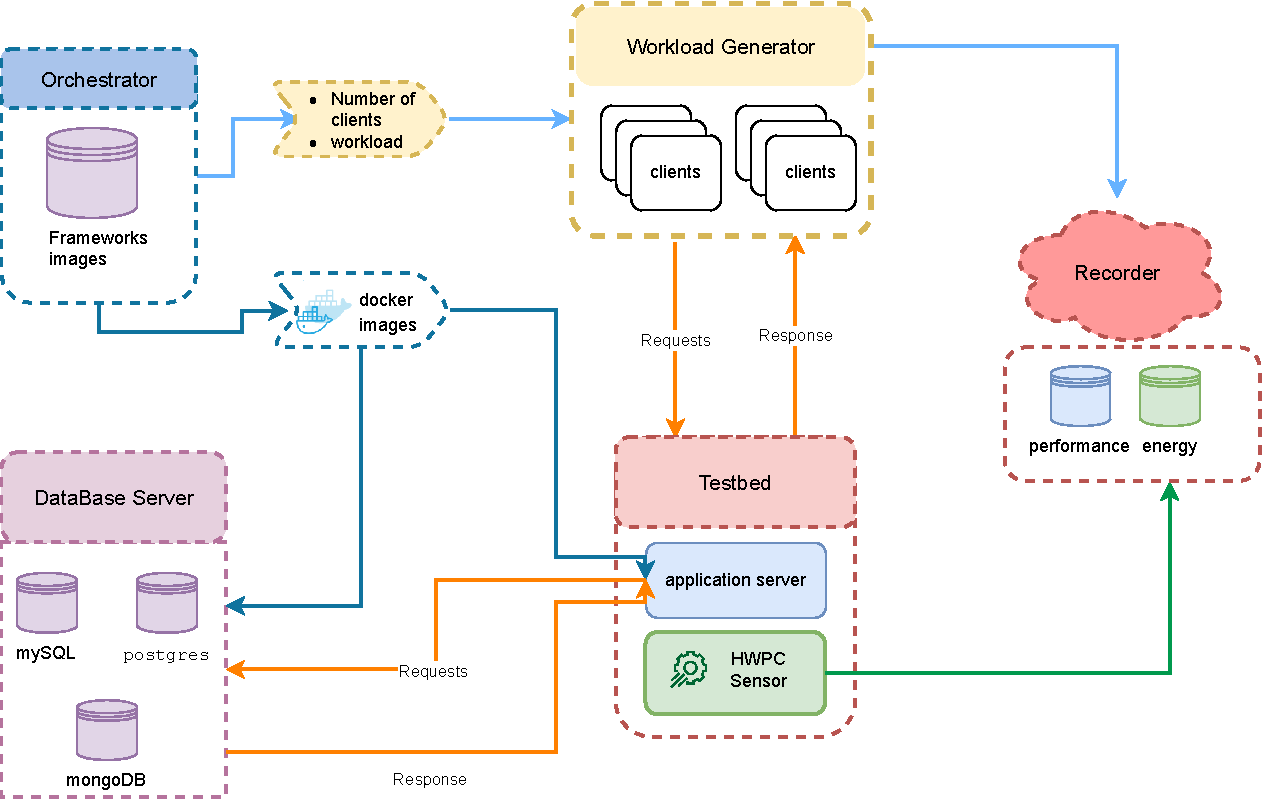
\includegraphics[width=.8\columnwidth]{imgs/architecture}
    \caption[Architecture]{Architecture of the experiments}
    \label{fig:architecture}
\end{figure}


\paragraph{Bias Analysis}
we are aware of bias analysis regarding the estimation of the total energy cost , the interference of other system processess during the execution and some external events. Thus, we run experiments multiple times and compute the average.

\subsection{Extension}
To follow the guidelines that we presented in chapter \ref{chapter:benchmarking} we provide a github repository \footnote{\url{https://github.com/chakib-belgaid/FrameworkBenchmarks}} where one can add extra \textbf{candidates} buy creating a new project using the option --new. then the they have just to fill the template and provide the docker image file.

to configure the \textbf{workload} we provide the option --concurrency-levels and --duration.
As for the choice of the database it is added in the docker image.


\section{Results \& Findings}
Overall we had $8,750$ tests, and all can be found in the repository.\footnote{\url{https://github.com/chakib-belgaid/frameworks-benchmarks-results}}
In this section, we will use the previous results to answer the following questions
\begin{itemize}
    \item is there a dominant programming language when it comes to performance, energy consumption, and latency ?
    \item which class of programming language is performing well ?
    \item ss there a correlation between energy consumption and latency ?
    \item is there an impact on the server when it comes to changing the database?
\end{itemize}

Since most of the companies use the same stack, we won't be aggregating the results since it may lead to confusion.
For example, comparing the average energy consumption of each programming language will not reflect reality, particularly when we have two frameworks on opposite ends of the spectrum. 

\subsection{Overall all statistics}
In order to determine which framework/stack is performing well we need to establish some general idea about the average In order to determine which framework/stack is performing well, we need to establish some general idea about the average energy consumption and latency of the frameworks. Instead of giving just the raw energy consumption of those frameworks, we will provide some green factors to determine which one is eco-friendly and which one is greedy.
In this part, we will discuss the average behavior of the frameworks, highlight some tendencies, and eliminate the outliers.
As we said in the threats to validity, being an outlier in this case does not mean that the framework is not performing well; it just means that the framework is not performing well in the same way as the others within the context of this experiment.

On the other hand the cost a single request is proportionate to the number of requests per second of the framework 

To narrow the research space, we will look for a correlation between the metrics. The Pearson correlation coefficient~\cite{zar2005spearman} will be used to determine this correlation. Because the Shapiro-Wilk~\cite{shapiro1968comparative} test yielded a p-value of 0.0 for all metrics.

Figre \ref{fig:correlation} depicts the correlation between the metrics. The Pearson correlation coefficient quantifies the linear correlation between two variables X and Y. It ranges from -1 to +1, with 1 being total positive linear correlation, 0 representing no linear correlation, and -1 representing whole negative linear correlation. The stronger the correlation, the closer the value is to 1 or -1. The weaker the correlation, the closer the value is to zero. The Pearson product-moment correlation coefficient is another name for the correlation coefficient. This correlation coefficient is also known as the Pearson product-moment correlation coefficient.
One can notice that there is a strong correlation between the energy consumption of the CPU  and the DRAM .Therefore we will exculde the DRAM metric from our study. 

intersently there is no correlation between the energy consumption of the CPU and the latency, which means that we can achieve both a low latency and a low energy consumption at the same time. 
%  TODO : add example of two programming langauges that have low latency and low energy consumption 
\begin{figure}[bht]
    \centering
    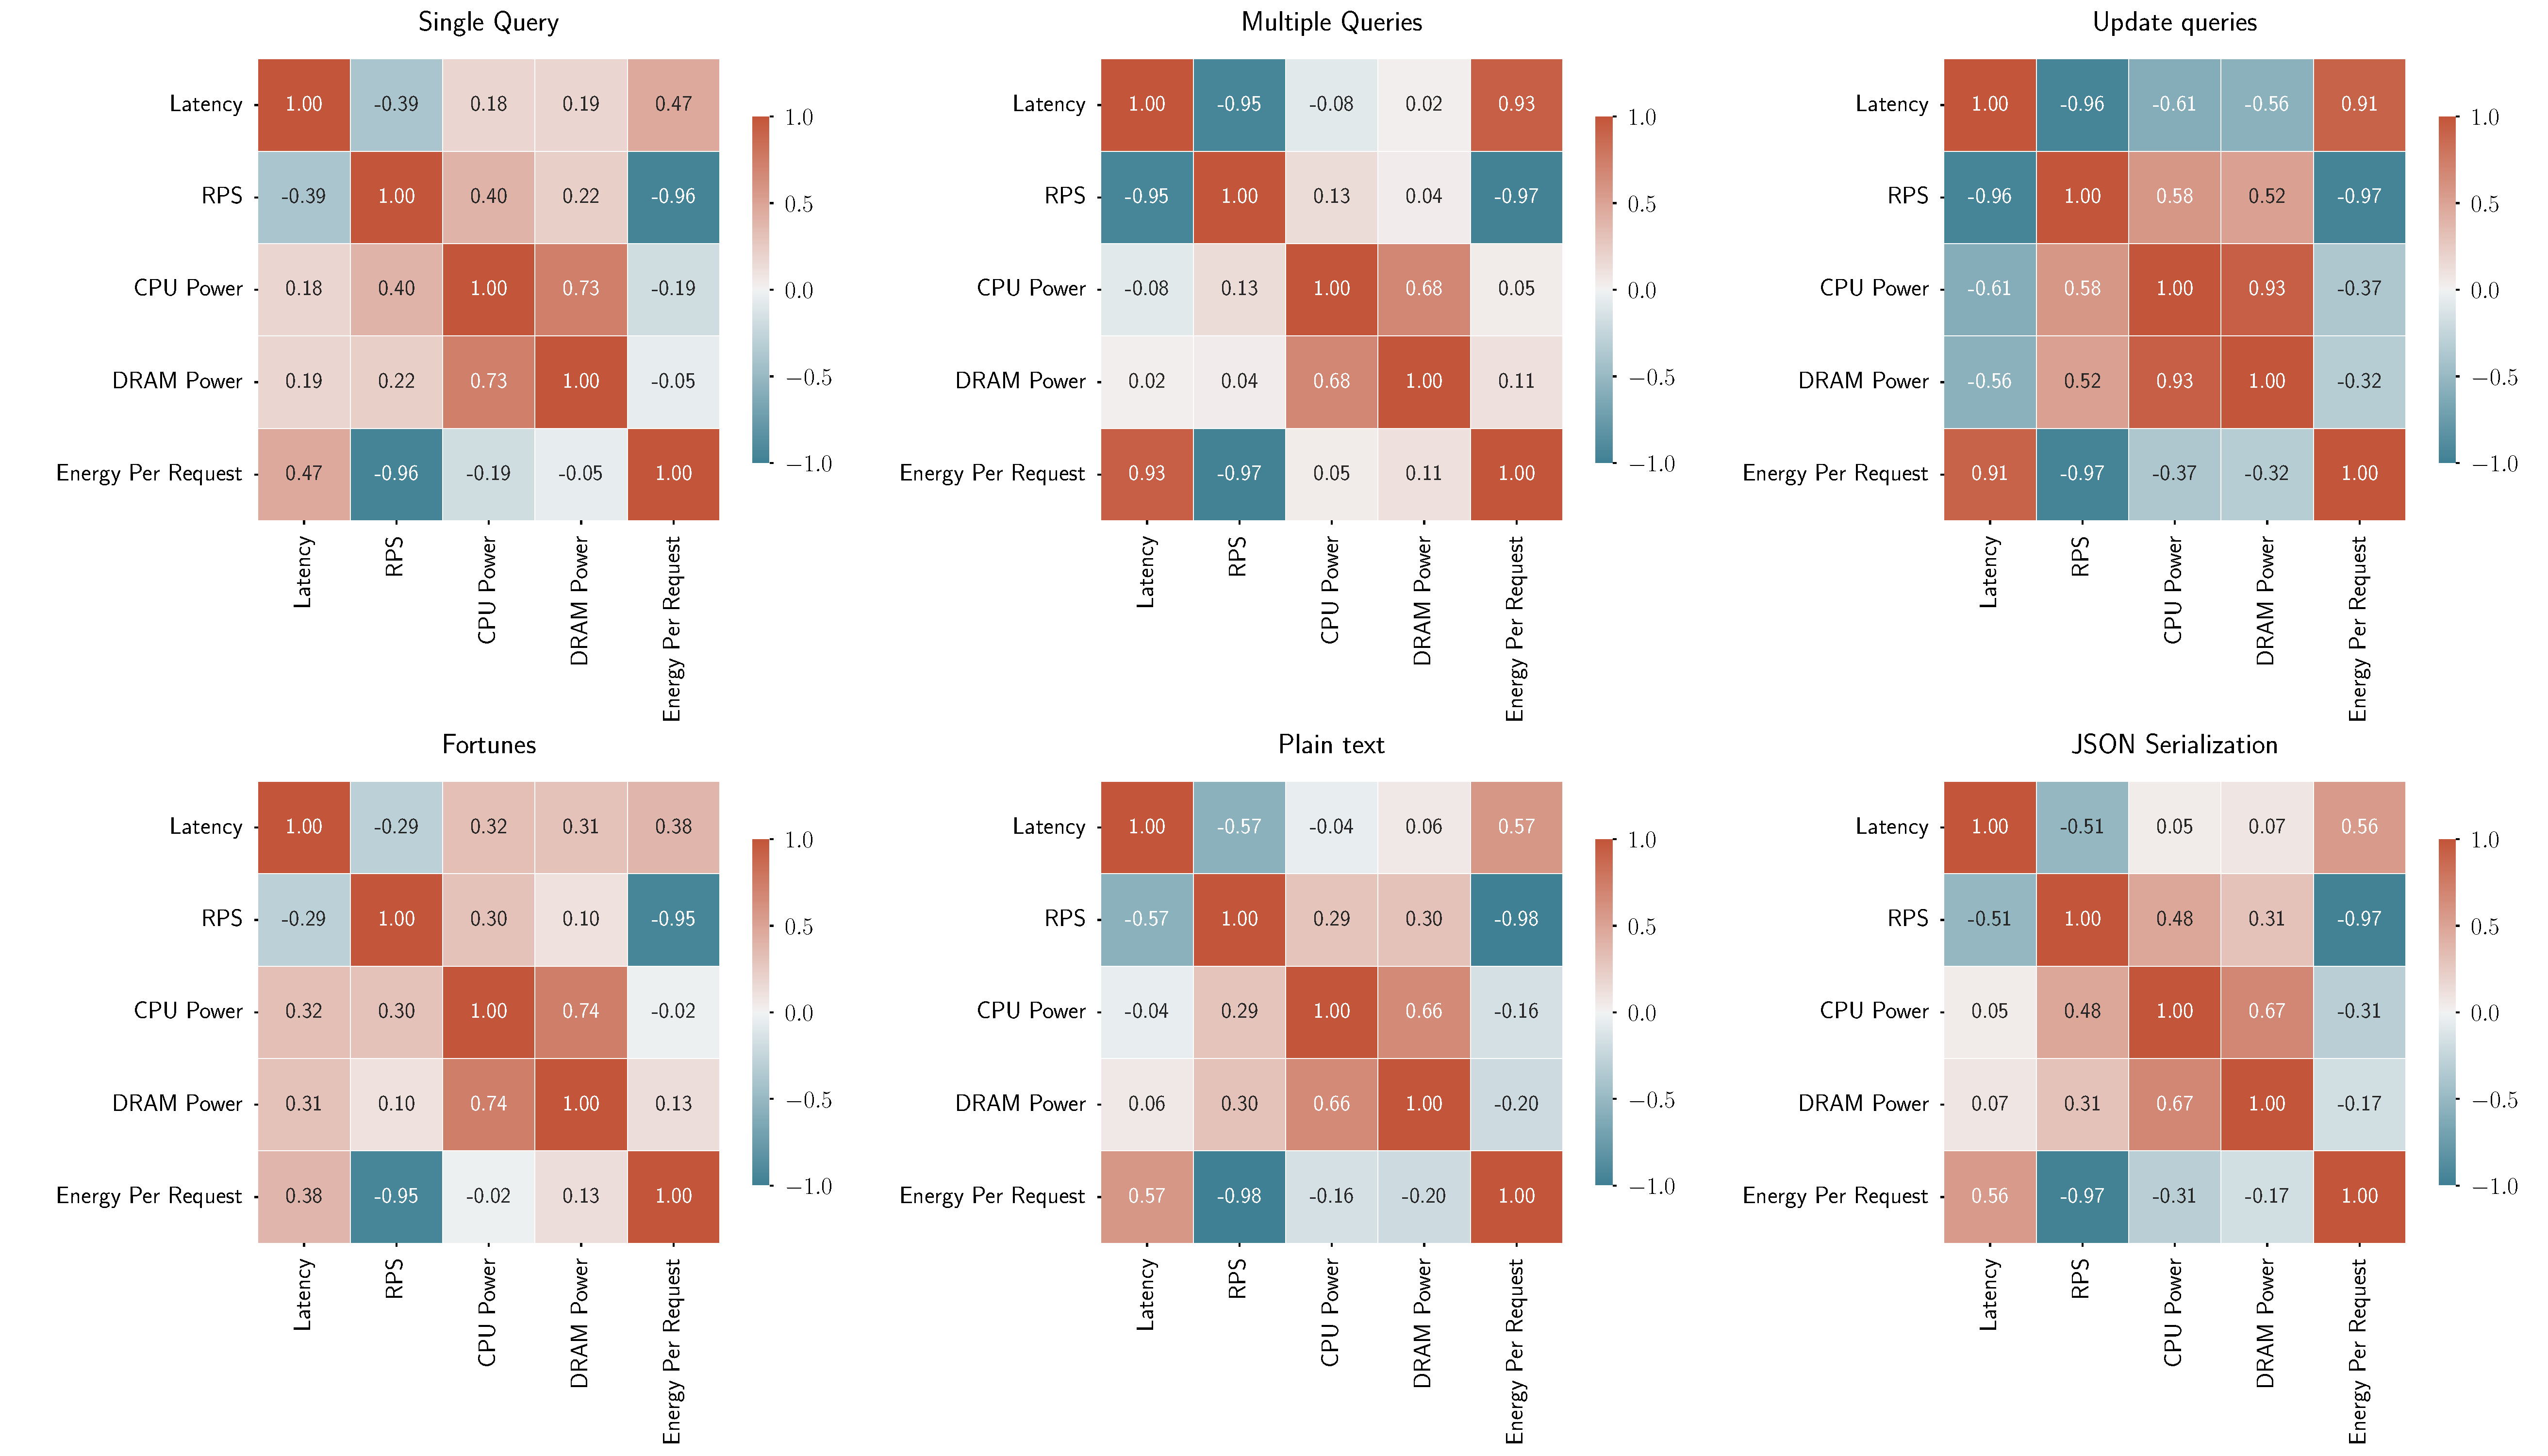
\includegraphics[width=.8\columnwidth ]{imgs/correlation_all}
    \caption{Spearman Rank Correlation between different metrics}
    \label{fig:correlation}
\end{figure}


then we group the implementation by the compiling type ,therefore we will have.
\begin{itemize}
    \item compiled languages 
    \item interpreted languages
    \item JVM-based languages 
    \item .net-based languages
    \item other VM-based languages
\end{itemize}


\begin{figure}[bht]
    \centering
    \caption{Average power consumption for the Single query test}
    \label{fig:av_power_db}
    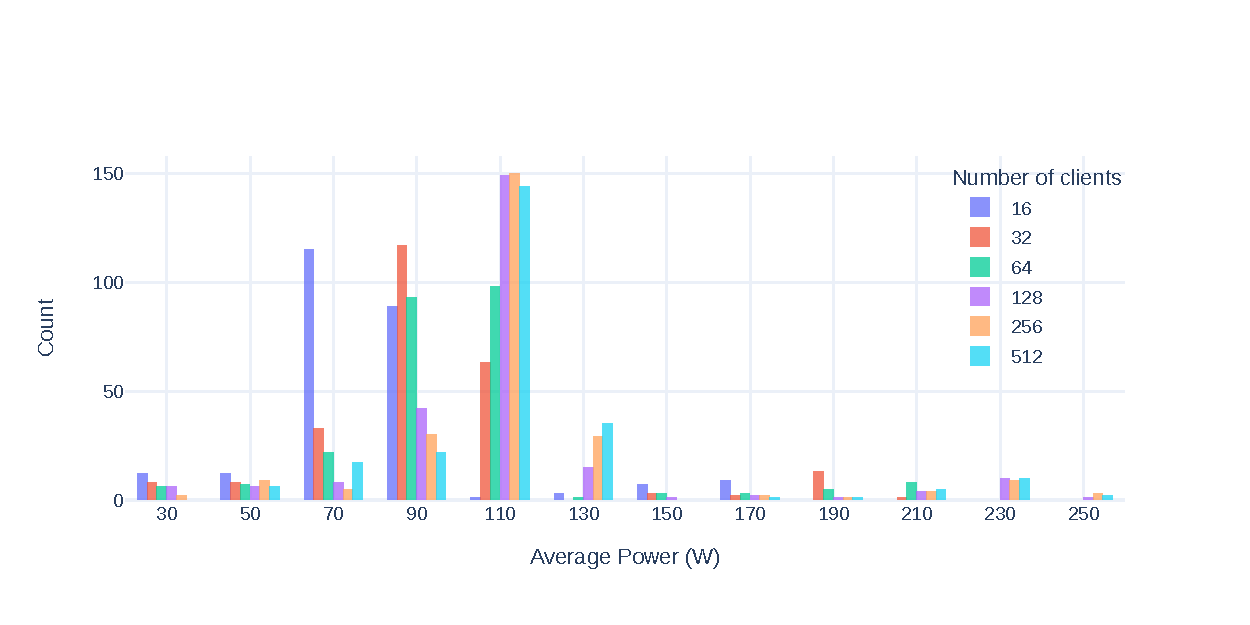
\includegraphics[width=.8\columnwidth]{imgs/av_power_db}

\end{figure}


\begin{figure}[bht]
    \centering
    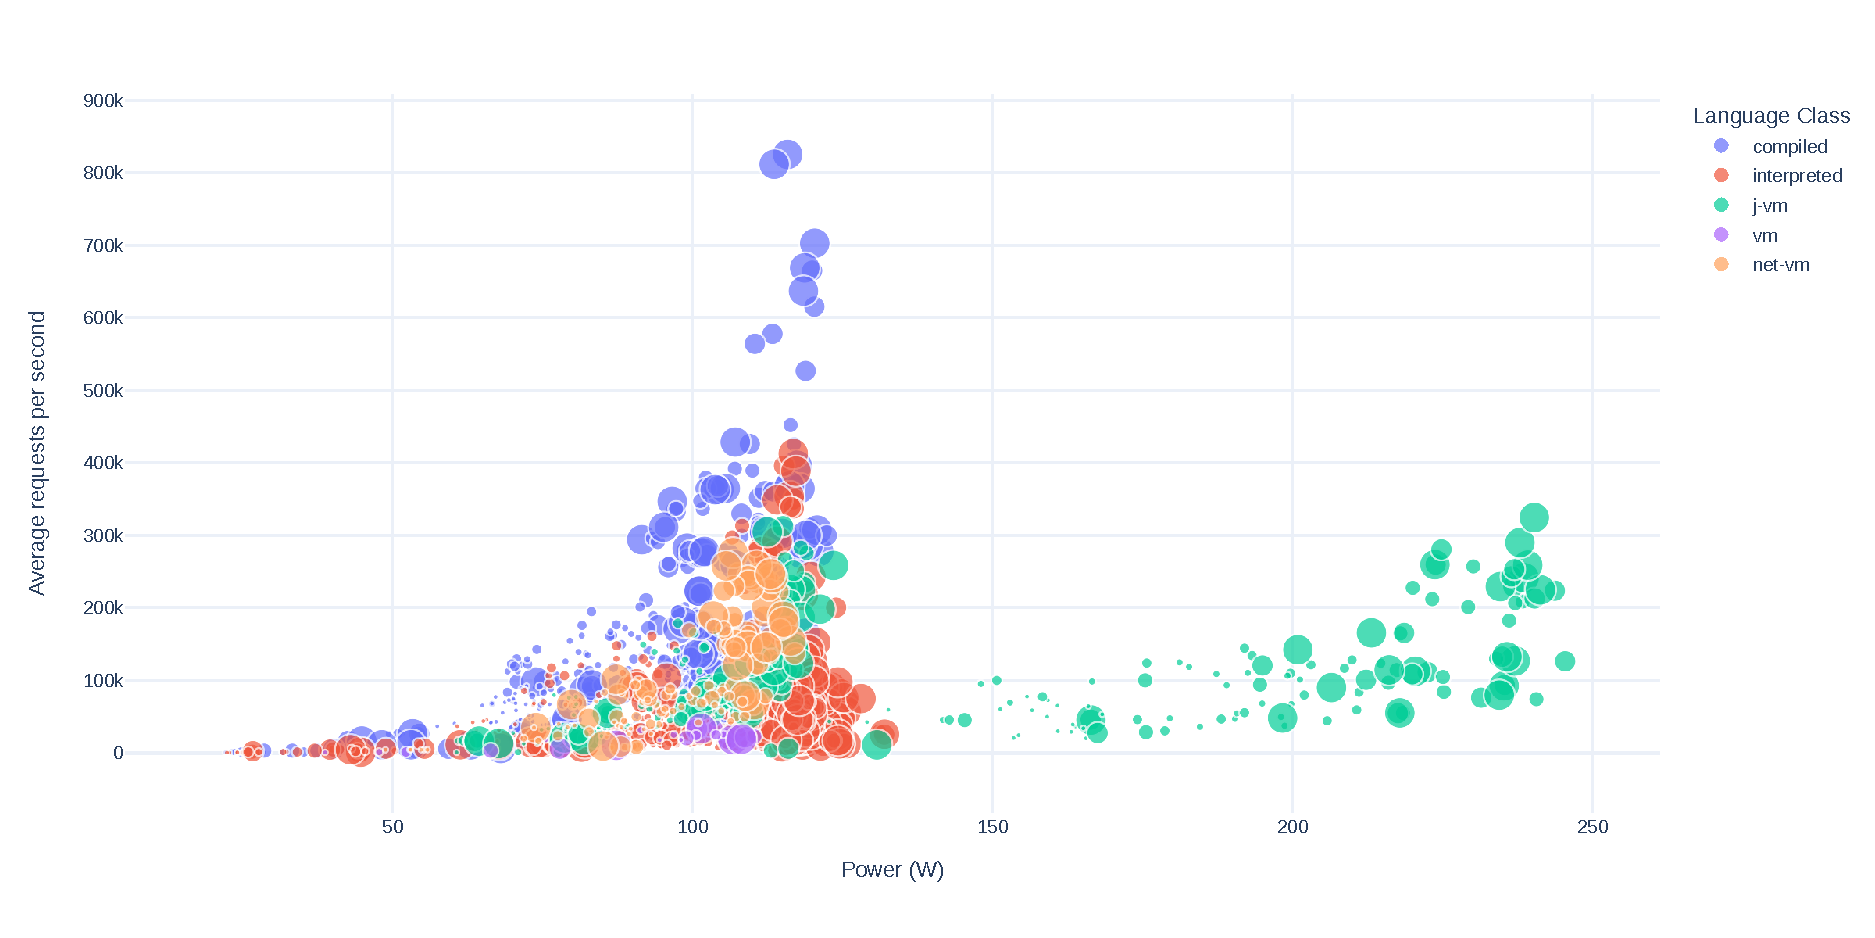
\includegraphics[width=
        \columnwidth]{imgs/power_requests_db}
    \caption{total request vs average power consumption for the Single query test ( size of circles represents the number of clients)}
    \label{fig:power_requests_db}
\end{figure}
\begin{figure}[bht]
    \centering
    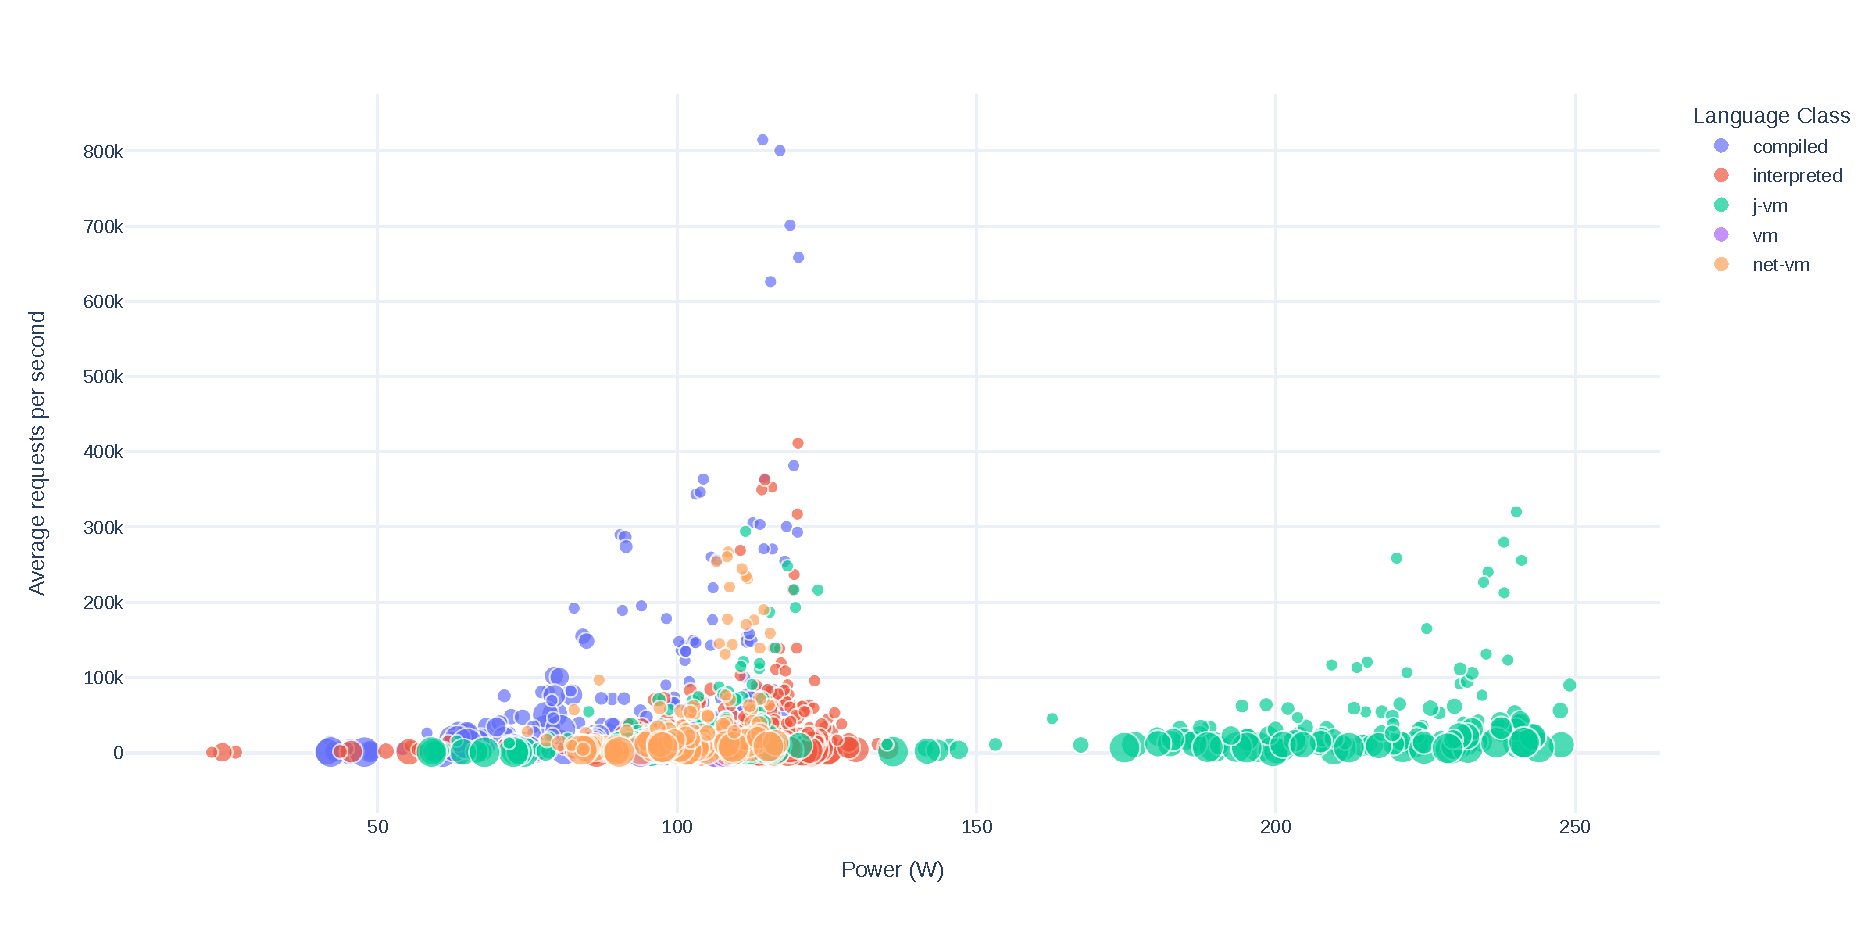
\includegraphics[width=
        \columnwidth]{imgs/power_requests_query}
    \caption{total request vs average power consumption for the multiple queries test ( Size of circles represents the size of the query )}
    \label{fig:power_requests_query}
\end{figure}
\begin{figure}[bht]
    \centering
    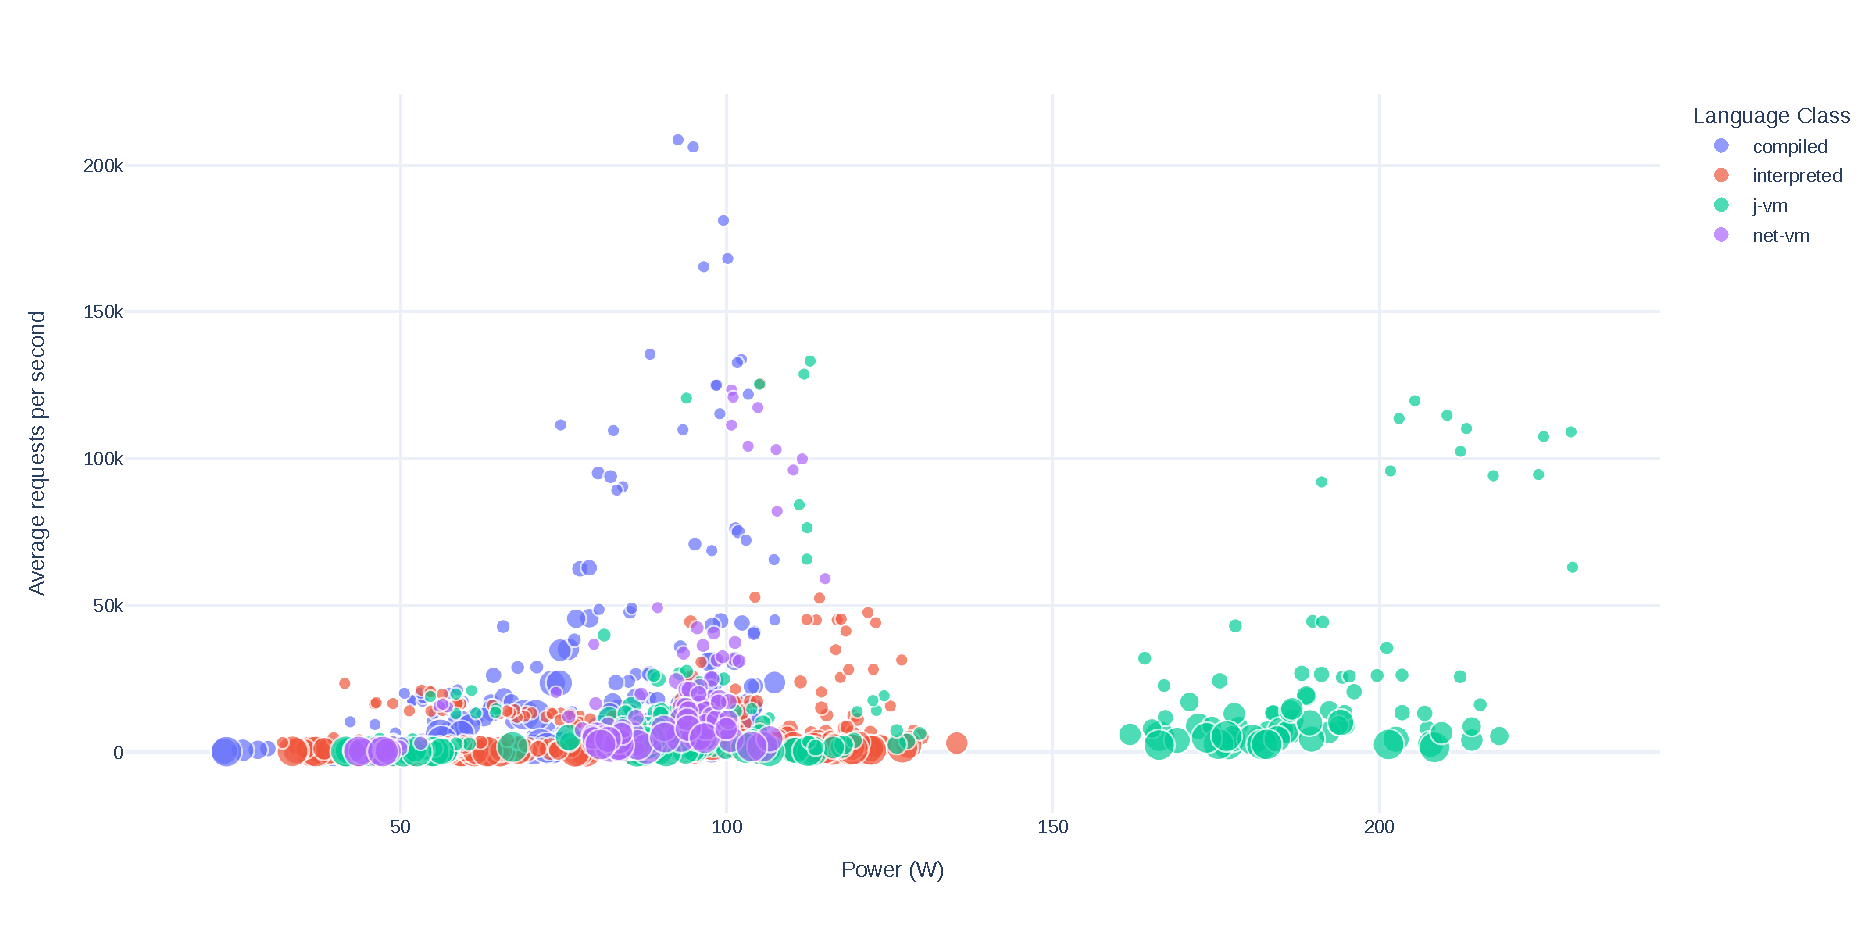
\includegraphics[width=
        \columnwidth]{imgs/power_requests_update}
    \caption{total request vs average power consumption for the update queries test ( Size of circles represents the size of the query )}
    \label{fig:power_requests_update}
\end{figure}
\begin{figure}[bht]
    \centering
    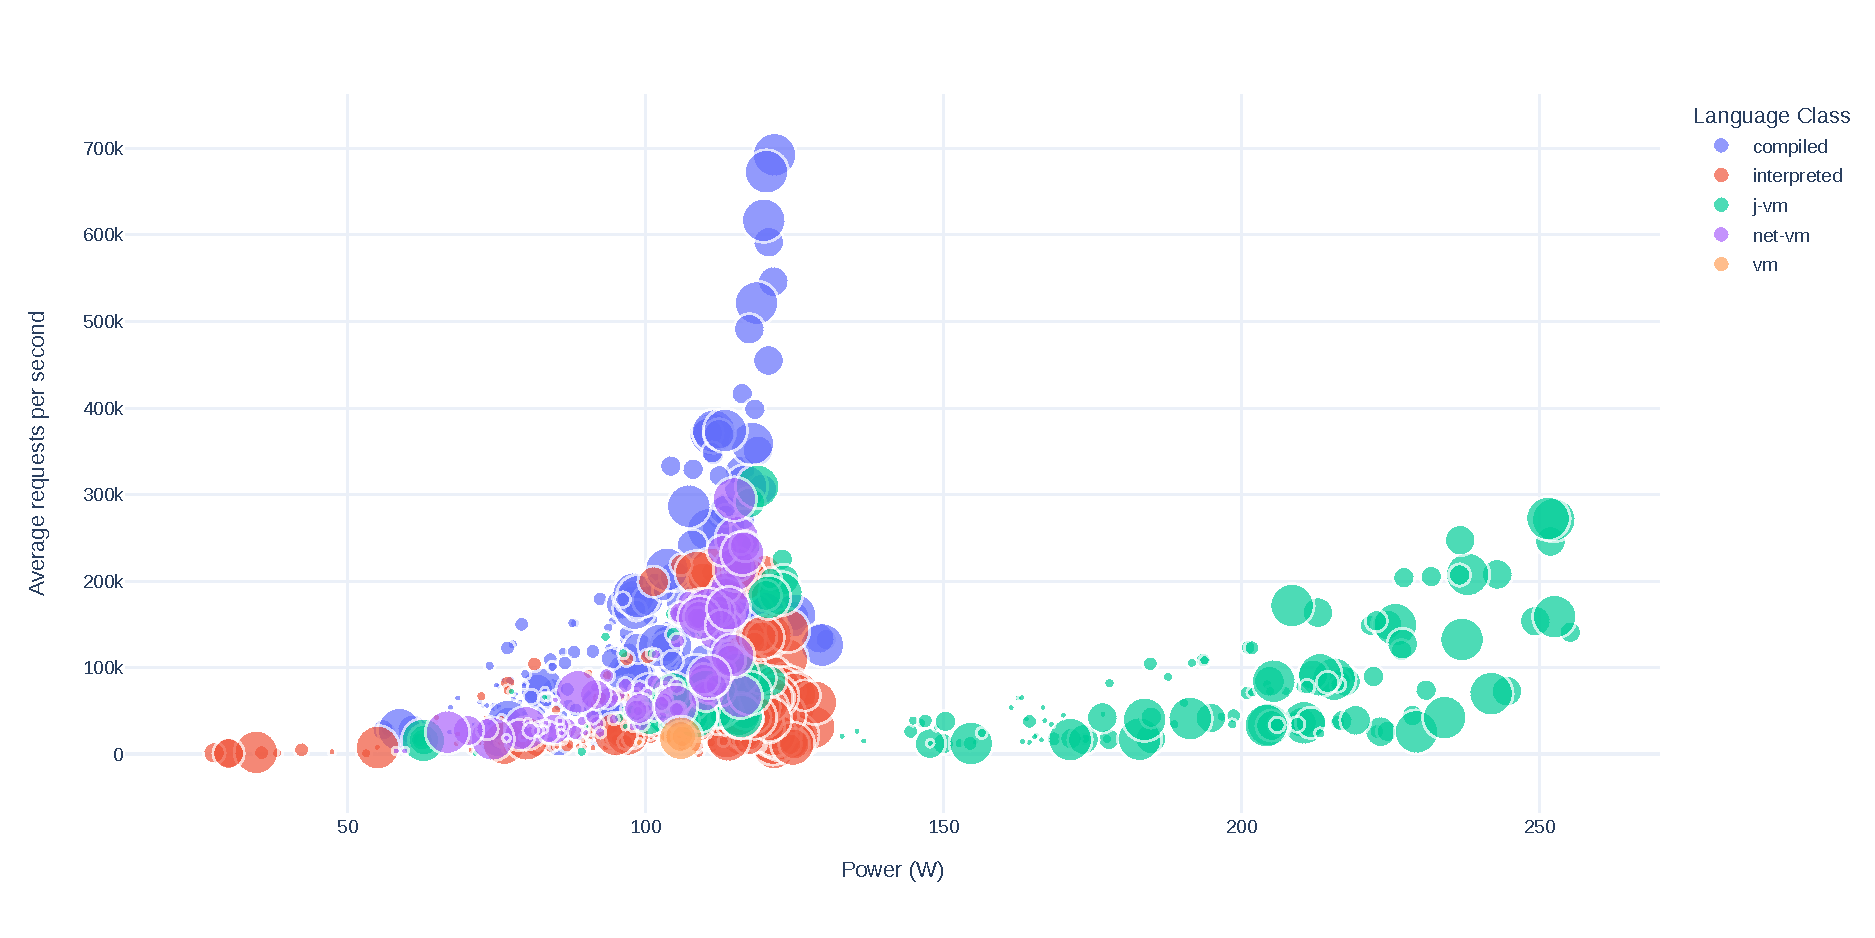
\includegraphics[width=
        \columnwidth]{imgs/power_requests_fortune}
    \caption{total request vs average power consumption for Fortunes test ( Size of circles represents the number of clients)}
    \label{fig:power_requests_fortune}
\end{figure}
\begin{figure}[bht]
    \centering
    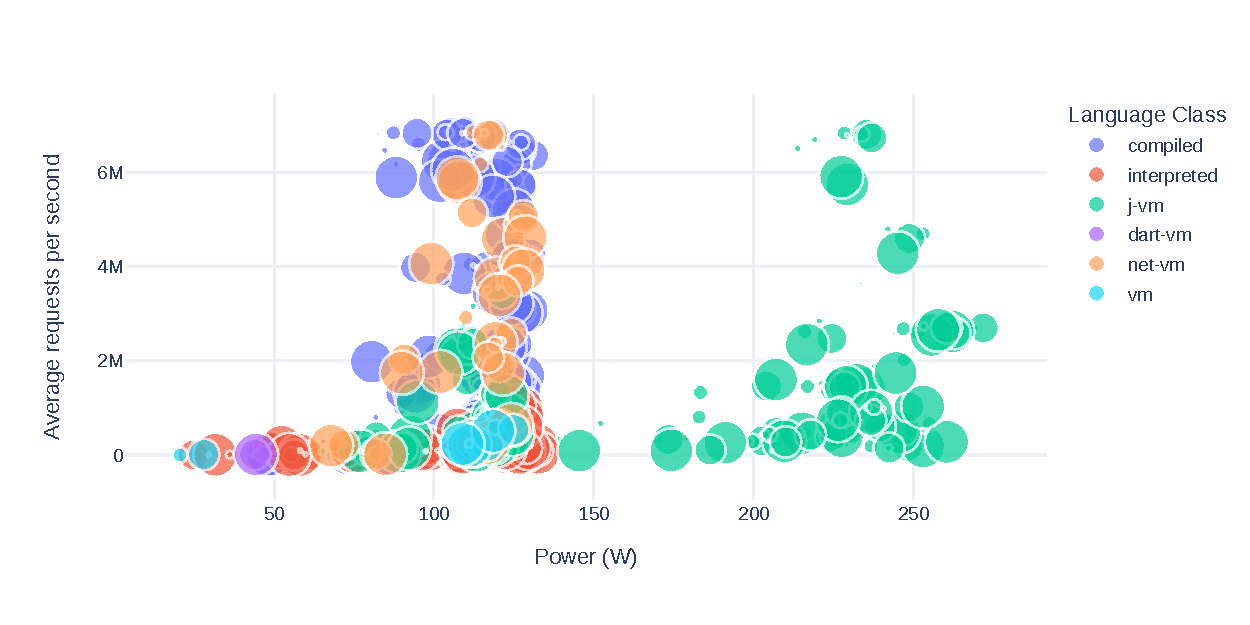
\includegraphics[width=
        \columnwidth]{imgs/power_requests_plaintext}
    \caption{total request vs average power consumption for plainText test ( size of circles represents the number of clients)}
    \label{fig:power_requests_plaintext}
\end{figure}
\begin{figure}[bht]
    \centering
    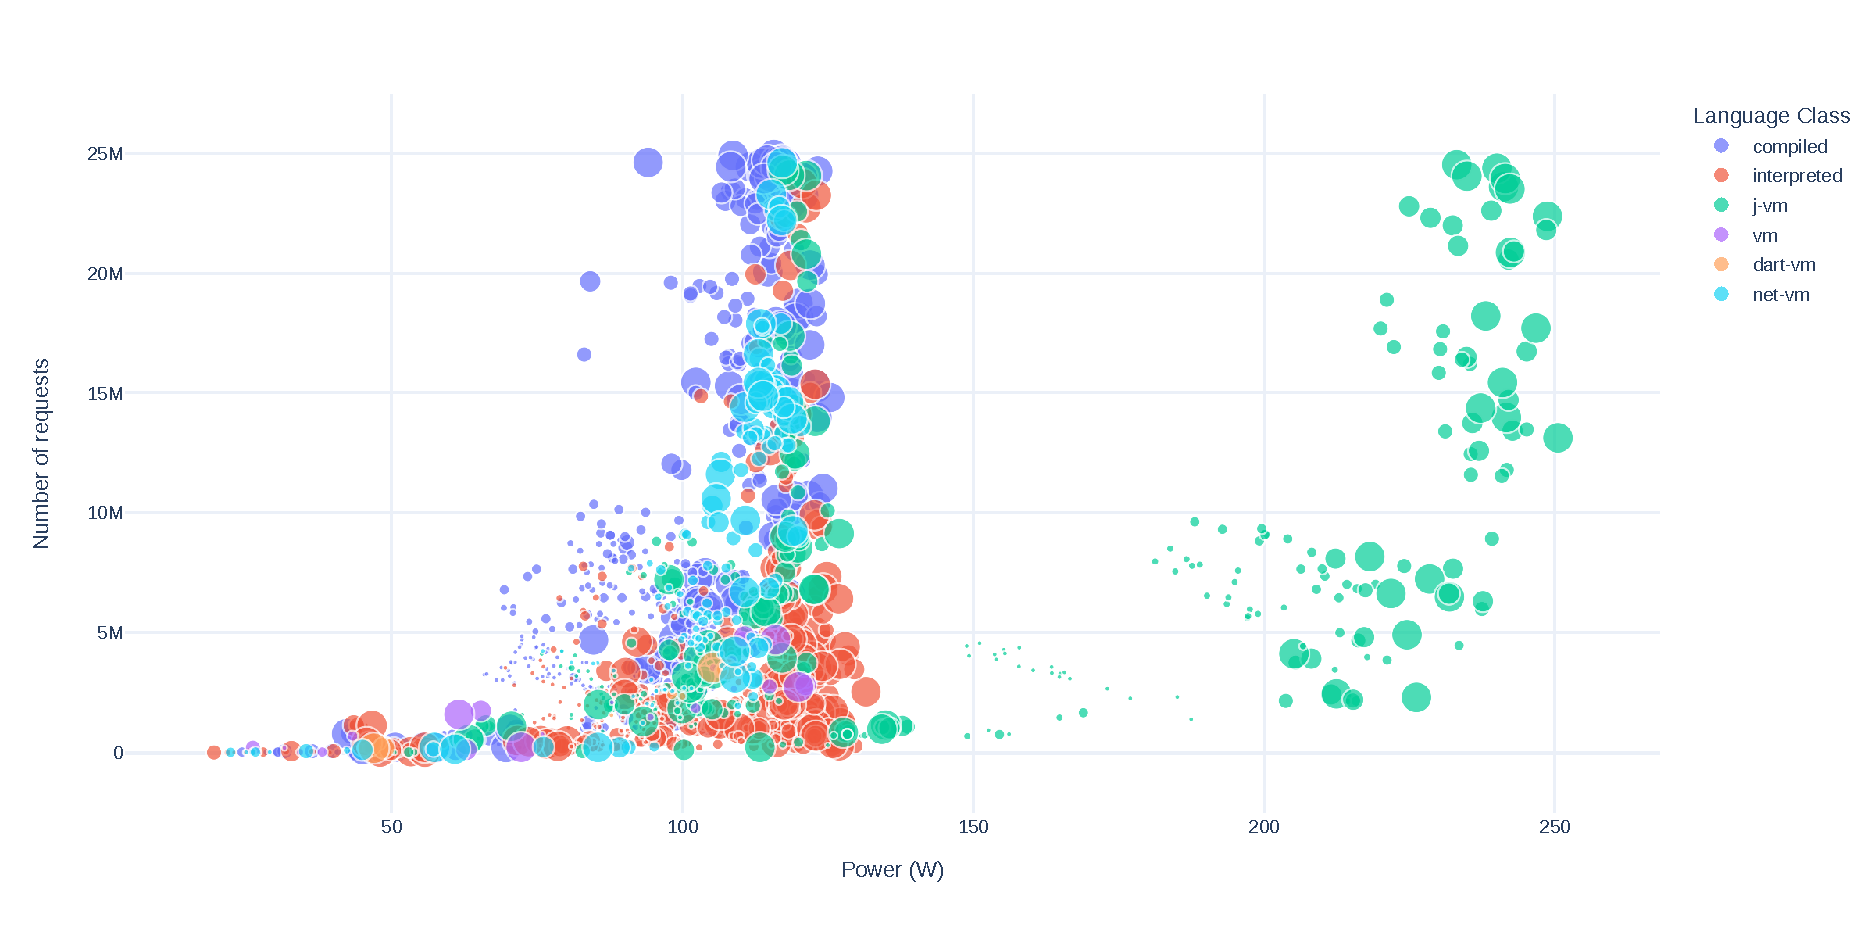
\includegraphics[width=
        \columnwidth]{imgs/power_requests_json}
    \caption{total request vs average power consumption for JSON Serialization test ( size of circles represents the number of clients)}
    \label{fig:power_requests_json}
\end{figure}
% to reduce the space of research we will be looking for some correlation 
% same thing for the number of clients , mayebe we gonna consider 3 cases - 0 , low and high 

%  when comparing static vs dynamic programming langauges we exclude the ones that uses reflection aka C# and JAVA

%% for more about the syntax we recommand cheking this website https://learnxinyminutes.com/



\section{Threats to Validity}
We are aware of the bias inducted by the implementation of a candidates, therefore we propose  the framework ( see the part of extension) to allow the readers to confirm themselves any new hypothesis. regarding a new framework , an new workload a new database ..etc

% \subsection{tools}
